% Created 2018-06-25 Mo 13:07
% Intended LaTeX compiler: pdflatex
\documentclass[11pt]{scrartcl}
\usepackage[utf8]{inputenc}
\usepackage[T1]{fontenc}
\usepackage{graphicx}
\usepackage{grffile}
\usepackage{longtable}
\usepackage{wrapfig}
\usepackage{rotating}
\usepackage[normalem]{ulem}
\usepackage{amsmath}
\usepackage{textcomp}
\usepackage{amssymb}
\usepackage{capt-of}
\usepackage{hyperref}
\usepackage[framemethod=TikZ]{mdframed}
\usepackage[authoryear,round]{natbib}
\title{Response to reviewer 1}
\date{}
\hypersetup{
 pdfauthor={Simon Pfreundschuh},
 pdftitle={},
 pdfkeywords={},
 pdfsubject={},
 pdfcreator={Emacs 24.5.1}, 
 pdflang={English}}

\RequirePackage[normalem]{ulem} %DIF PREAMBLE
\RequirePackage{luacolor}\definecolor{RED}{rgb}{1,0,0}\definecolor{BLUE}{rgb}{0,0,1} %DIF PREAMBLE
\providecommand{\DIFadd}[1]{{\protect\textcolor{blue}{\uwave{#1}}}} %DIF PREAMBLE
\providecommand{\DIFdel}[1]{{\protect\textcolor{red}{\sout{#1}}}}                      %DIF PREAMBLE
%DIF SAFE PREAMBLE %DIF PREAMBLE
\providecommand{\DIFaddbegin}{} %DIF PREAMBLE
\providecommand{\DIFaddend}{} %DIF PREAMBLE
\providecommand{\DIFdelbegin}{} %DIF PREAMBLE
\providecommand{\DIFdelend}{} %DIF PREAMBLE
%DIF FLOATSAFE PREAMBLE %DIF PREAMBLE
\providecommand{\DIFaddFL}[1]{\DIFadd{#1}} %DIF PREAMBLE
\providecommand{\DIFdelFL}[1]{\DIFdel{#1}} %DIF PREAMBLE
\providecommand{\DIFaddbeginFL}{} %DIF PREAMBLE
\providecommand{\DIFaddendFL}{} %DIF PREAMBLE
\providecommand{\DIFdelbeginFL}{} %DIF PREAMBLE
\providecommand{\DIFdelendFL}{} %DIF PREAMBLE

\newenvironment{change}[1][]{%
  \begin{mdframed}[frametitle={Line #1:}]%
}{%
  \end{mdframed}%
}

\begin{document}
\maketitle

\setlength{\parindent}{0cm}

We thank the referee for the time he/she has put on reading our manuscript and providing
feedback.

Based on the combined comments of the referees, we have decided to implement these general
changes:

\begin{itemize}
\item We will switch to an airborne measurement set-up and
  the introduction section will be modified accordingly
\item The text in the result section will be shortened significantly
\item Redundant results for scene 2 will be placed in an appendix
\item The selection of tested retrieval habits will be revised/changed
\end{itemize}

Below we respond to the main questions raised by the referee, and outline how we will
revise the manuscript.

\section{General comments}

\subsection*{Reviewer comment 1}

As noted in Section 4.2.4, the a priori assumptions do not describe reality very
well. In particular, I suspect that the information content of Dm and N0* is
highly dependent on the a priori assumptions of these two variables in the
retrieval framework. Especially with a radar measurement, since Z is sensitive
to both parameters over a wide range of the parameter space, the relative
sensitivity and therefore information content will almost entirely depend on the
relative constraints on these parameters imposed by Xa and Sa. As such it is
imperative to accurately characterize these. I understand the choice to use the
DARDAR constraints, but it’s clear from the cross-section plots that the model
ice particle concentrations vary over a much wider range than the roughly 2
orders of magnitude that Eq. 4 provides over a 220-272 K temperature range. So,
when the retrieval results are compared to model “reality”, it seems that a lot
of N0* variability is folded into Dm and this is especially evident in Figures
13 and 14. My overall concern is that it is difficult to interpret some of the
results when the model fields and the a priori assumptions differ so strongly.

\subsubsection*{Author response:}

To avoid potential misunderstanding we would like to point out that the
variation of the a priori mean with temperature, which is given by Eq. 4, does
not limit the retrieved values of $N_0^*$ to this range. How much $N_0^*$ is
allowed to vary around the a priori mean is determined by the covariance matrix.
Since the standard deviation for $\text{log}_{10}(N_0^*)$ at each grid point was
set to $2$ (c.f. Tab.~3), $N_0^*$ is free to vary over several orders of
magnitude in addition to the variation of the a priori profile.

Furthermore, the sentence in Section~4.2.4 was badly formulated and did not
really express what we wanted to say here. The a priori assumptions are not
generally bad for the model (after all the averaged results for the first scene
are good). Rather, they are insufficient to accurately describe the (co-)variability
of $D_m$ and $N_0^*$.

Nonetheless, the point raised by the reviewer certainly remains valid: In
absolute terms, the interpretation of the retrieval results is dependent on the
a priori assumptions. We argue here, however, that by applying equivalent a
priori assumptions in all retrievals, we can still derive conclusions on the
benefits of the combined retrieval approach based on a relative interpretation
of the retrieval results. In particular, our results indicate that the combined
retrieval has to rely less on a priori assumptions than the radar-only
retrieval. 

To address the issues raised by the reviewer we propose to make the following
changes in the manuscript:

\begin{itemize}
\item To extend the discussion of the role of the a priori (around L. 491) and
  its impact on the results.
\item To add a paragraph to the discussion of the limitations of the study (around L. 549)
  which clearly states that the retrieval results should not be interpreted in absolute terms
\item To rephrase the sentence in Sect. 4.2.4 (L. 545) to stress that is refers to the
  Gaussian nature of the a priori rather then the a priori itself.
\end{itemize}


%To address the issue raised by the reviewer, we propose the following
%changes to the manuscript:
%
%\begin{itemize}
%\item To make the role of the a priori clearer the discussion of the a priori
%  assumptions will be rewritten:
%
%\begin{change}[491]
%\DIFdelbegin \DIFdel{The a priori assumptions which were used in this study were similar but not
%identical to what is used in the DARDAR retrievals. Also here it should be
%noted, that the presented results should not be taken to be representative for
%the DARDAR product. Rather than this, the DARDAR a priori settings were chosen
%since they represent well established and validated assumptions for ice cloud
%retrievals and therefore should provide a reasonable starting point for the
%development of a combined cloud retrieval. The fact that the a priori
%assumptions used in the DARDAR retrieval do not agree with the microphysical
%properties of ice and snow in the GEM model, does not say much about the general
%validity of these assumptions.
%}%DIFDELCMD < 
%
%\DIFadd{The a priori assumptions used in this study are based on the DARDAR-CLOUD
%product, since they represent well established and validated assumptions for ice
%cloud retrievals. The role of the a priori is to complement the observations
%with additional information required to make the retrieval problem tractable.
%For the hydrometeor retrieval this means that the a priori determines how the
%information from the observations, which alone is insufficient to accurately
%determine both degrees of freedom of the PSD, is distributed between its $D_m$
%and $N_0^*$ parameters. For the radar-only retrieval, this works well for cloud
%systems containing both ice and snow but leads to biased retrievals in both IWC
%and IWP when this is not the case, as seen in Fig.~\ref{fig:results_boxes}.
%These problems could be remedied by introducing more specific a priori
%assumptions. However, these will be dependent on the cloud and hydrometeor type
%imposing the question of how these can be determined a priori. For the combined
%retrieval, however, this may not be necessary since the increased information
%content makes it less dependent on the a priori to infer the microphysical
%properties of the cloud.
%}\DIFaddend 
%\end{change}
%
%\item The statement from Section~4.2.4 on the a priori assumptions is corrected:
%
%\begin{change}[544]
%The forward model is non-linear and \DIFdelbegin \DIFdel{the assumed }\DIFdelend \DIFaddbegin \DIFadd{it is difficult to describe the variability
%of cloud parameters using }\DIFaddend Gaussian a priori assumptions\DIFdelbegin \DIFdel{do
%not describe reality very well}\DIFdelend .
%\end{change}
%
%\item A paragraph is added to Section~4.2.5 emphasizing that the results should
%  not be interpreted in absolute terms:
%
%\begin{change}[549]
%\DIFdelbegin \DIFdel{Finally, it is important to consider the limitations }\DIFdelend \DIFaddbegin \DIFadd{An important limitation }\DIFaddend of this study \DIFdelbegin \DIFdel{. The }\DIFdelend \DIFaddbegin \DIFadd{is its scope: The aim here was not to develop
%a production-ready combined retrieval product but rather a proof-of-concept to
%explore the observational approach. The retrieval }\DIFaddend results presented here \DIFdelbegin \DIFdel{are }\DIFdelend \DIFaddbegin \DIFadd{should
%therefore not be interpreted in absolute terms. The primary results are based on
%the relative performances of the three retrieval methods: Given equivalent a
%priori assumptions, the combined retrieval demonstrates higher sensitivity to
%the microphysical properties than the radar-only retrieval and lower errors
%in terms of IWC than the passive-only retrieval.
%}
%\end{change}
%
%\end{itemize}

\subsection*{Reviewer comment 2}

Forward model error is introduced when the different species present in the
model microphysics are combined into one species and when different scattering
models are used to represent the ice particles. That this is not represented in
Se could lead to over-fitting and poor convergence (I suspect this is part of
the reason why the normalized cost is much higher for the radiometer-including
retrievals). It should be relatively easy to quantify this error by re-running
the simulations with the retrieval assumptions(combining ice species, different
scattering models), and I suspect that this error term would dominate the
instrument noise term for many channels.

\subsubsection*{Author response}

It is certainly true that the simplified forward model used in the retrieval
introduces a forward modeling error and that it will likely dominate the sensor
noise. However, we do not agree with the reviewer that this is easy to quantify.
First of all, the error will not be Gaussian and will depend on the cloud
composition and the assumed particle shape, so that a more sophisticated error
model would be required to describe the error accurately. Furthermore, fitting
such a model to the test scenes would likely yield overly optimistic results as
this would mean making use of information that would not be available for real
retrieval observations.

Because of these difficulties, we decided to not pursue this in this study.
However, since this is an important point to mention, we will add a paragraph
in the discussion to on this issue.

%be added to the discussion of the retrieval method:
%
%\begin{change}[548]
%\DIFaddbegin \DIFadd{Some of the above-mentioned problems could likely be counteracted by accounting
%for the forward model error caused by the simplified forward model applied in
%the retrieval. However, finding an accurate description of this error
%would require developing a suitable model for it which was deemed out of the
%this studies' scope.
%\DIFaddend 
%}
%\end{change}


\section{Specific comments}

\subsection*{Reviewer comment 1}
Lines 85-88: I recommend the use of geographical spatial references
(i.e.,north/south rather than left/right)

\subsubsection*{Author response}

The proposed change will be adopted in the revised version of the manuscript.

%by introducing
%the following changes:
%
%\begin{change}[85]
%... retrieval. The first test scene, shown in panel (a), is located in the
%  tropical Pacific and contains a convective storm system in the \DIFdelbegin
%  \DIFdel{right }\DIFdelend \DIFaddbegin \DIFadd{northern }\DIFaddend half of
%  the scene and its anvil that extends into the \DIFdelbegin \DIFdel{left
%  }\DIFdelend \DIFaddbegin \DIFadd{southern }\DIFaddend half of the scene. The
%  second scene, shown in panel (b), is located in the North Atlantic and
%  contains an ice cloud in the \DIFdelbegin \DIFdel{first quarter }\DIFdelend
%  \DIFaddbegin \DIFadd{southern part }\DIFaddend and a low-level, mixed-phase
%  cloud in the remainder of the scene.
%\end{change}


\subsection*{Reviewer comment 2}

Line 98 (also 176,252,449): Instead of vertical/horizontal (which are
dependent on the convention used for plotting), I recommend the use of
concentration/size tocharacterize the dimensions of the particle size
distribution.

\subsubsection*{Author response}

The proposed change will be adopted in the revised version of the manuscript.

%The proposed changes will be adopted in the revised version of the manuscript
%by introducing the following changes:
%
%\begin{change}[97]
%\ldots simulations. As these plots show, the
%assumed particle size distributions across different ice species vary mostly in
%their \DIFdelbegin \DIFdel{horizontal and vertical scaling }\DIFdelend \DIFaddbegin \DIFadd{scaling with respect to size and concentration}\DIFaddend , whereas the function \ldots
%\end{change}
%
%\begin{change}[176]
%The PSD of a hydrometeor species at a \DIFdelbegin \DIFdel{given }\DIFdelend \DIFaddbegin \DIFadd{certain }\DIFaddend height level is
%\DIFdelbegin \DIFdel{represented by a vertical and a horizontal scaling parameter}\DIFdelend \DIFaddbegin \DIFadd{given by a generalized gamma distribution function with four parameters. Two of
%them}\DIFaddend , the mass-weighted mean diameter $D_m$\DIFaddbegin \DIFadd{, which scales the PSD along the size
%dimension, }\DIFaddend and the normalized number density $N_0^*$\DIFdelbegin \DIFdel{. Alternative 
%parametrizations using mass density and $D_m$ or the mass density and $N_0^*$
%have been tested but no considerable effect on retrieval performance has been
%observed.
%}%DIFDELCMD < 
%
%%DIFDELCMD < %%%
%\DIFdel{The retrieval computes vertical profiles of the two scaling parameters $D_m$ and
%$N_0^*$ for each of the two hydrometeor species. The remaining shape of each }\DIFdelend \DIFaddbegin \DIFadd{, which scales the particle
%  concentration, are retrieved. The \ldots}\DIFaddend
%\end{change}
%
%\begin{change}[252]
%The question that is addressed here is whether the combination of active and
%passive observations is able to constrain both the \DIFdelbegin \DIFdel{horizontal and the
%vertical scaling factors of the PSD }\DIFdelend \DIFaddbegin \DIFadd{size and concentration }\DIFaddend of the
%ice particles in the cloud. 
%\end{change}
%
%\begin{change}[449]
%The results show that the combined
%observations can simultaneously constrain the \DIFdelbegin \DIFdel{horizontal and vertical scaling of
%the particle size distribution}\DIFdelend \DIFaddbegin \DIFadd{size and concentration of
%particles in the cloud}\DIFaddend .
%\end{change}


\subsection*{Reviewer comment 3}

Line 100: A few more details on the Milbrant and Yau microphysics sheme that are
relevant to this study would be helpful here. For example: What is the assumed
shape(functional form) of the particle size distribution, and what are the
prognostic variables(e.g., number concentration, mixing ratio)?

\subsubsection*{Author response}

We will follow the reviewers comment and add the requested information
to the manuscript.

%To address the reviewers comment, the paragraph describing the Milbrandt-Yau microphysics scheme
%has been extended to provided the information demanded by the reviewer:
%
%\begin{change}[91]
%The GEM model uses \DIFaddbegin \DIFadd{a two-moment scheme with }\DIFaddend six types of hydrometeors to
%represent clouds and precipitation \citep{milbrandtyau05}: Two classes of liquid
%hydrometeors (rain and liquid cloud) and four of frozen hydrometeors (cloud ice,
%snow, hail and graupel). The particle size distribution (PSD) of each
%hydrometeor \DIFdelbegin \DIFdel{type is parametrized by its particle number concentration and mass density. The
%full
%particle size distributioncan be prognosed from the two moments using a
%species-dependent parametrization and
%}\DIFdelend \DIFaddbegin \DIFadd{class is described by a three-parameter gamma distribution. The
%prognostic parameters of the two-moment scheme are the slope and intercept
%parameters of the distribution, which are derived from the mixing ratios and
%number densities predicted by the GEM model. The third parameter of the PSD and
%the }\DIFaddend mass-size relationship \DIFaddbegin \DIFadd{of each hydrometeor class are set to fixed,
%class-specific values}\DIFaddend . The parameters of the mass-size \DIFdelbegin \DIFdel{relationship }\DIFdelend \DIFaddbegin \DIFadd{relationships }\DIFaddend are given
%in Tab.~\DIFdelbegin \DIFdel{\ref{tab:species_parameters}. As
%shown in the table, the }\DIFdelend \DIFaddbegin \DIFadd{\ref{tab:partice_properties}. The }\DIFaddend masses of all ice particles in the
%model are assumed to scale with a power of three, which leads to high densities
%for large particles.
%\end{change}

\subsection*{Reviewer comment 4}
Line 135: Does the ARTS radar solver also provide analytic Jacobians?

\subsubsection*{Author response}

Yes, it does. A sentence will be added to the description of the forward model
to clarify this.

%This is now also mentioned in the description of the retrieval forward model:

%\begin{change}[135]
%All simulations presented in this study were performed using Version 2.3.1245 of
%the Atmospheric Radiative Transfer Simulator (ARTS, \cite{arts18}). Radar
%reflectivities are computed using ARTS' built-in single-scattering radar solver\DIFaddbegin \DIFadd{,
%which provides analytic Jacobians}\DIFaddend . For \ldots
%\end{change}

\subsection*{Reviewer comment 5}
Line 187: “particles” should be “particle”

\subsubsection*{Author response}

The sentence will be removed in the revised version of the manuscript as it
the information it conveyed was not deemed relevant.

%\begin{change}[187]
%  \ldots rain drops. \DIFdelbegin \DIFdel{All calculations involving particles
%    size distributions use the volume-equivalent diameter $D_\text{eq}$ as size
%    variable.
%}%DIFDELCMD < 
%\end{change}


\subsection{Reviewer comment 6}
Line 198: Is Dm also only retrieved at these 10 points, or just N0* (and Dm retrievedin each radar range gate as in Grecu et al. 2016)?

\subsubsection*{Author response}

$D_m$ is actually retrieved at the resolution of the GEM model scenes. Since
questions about the retrieval grids were also raised by the other reviewers, we
will add an illustration of the grids applied in the different retrieval
configurations to the manuscript.

%To make
%this more clear the following sketch will be added in the beginning of the
%section describing the retrieval setup:

%  \begin{figure}
%\begin{center}
%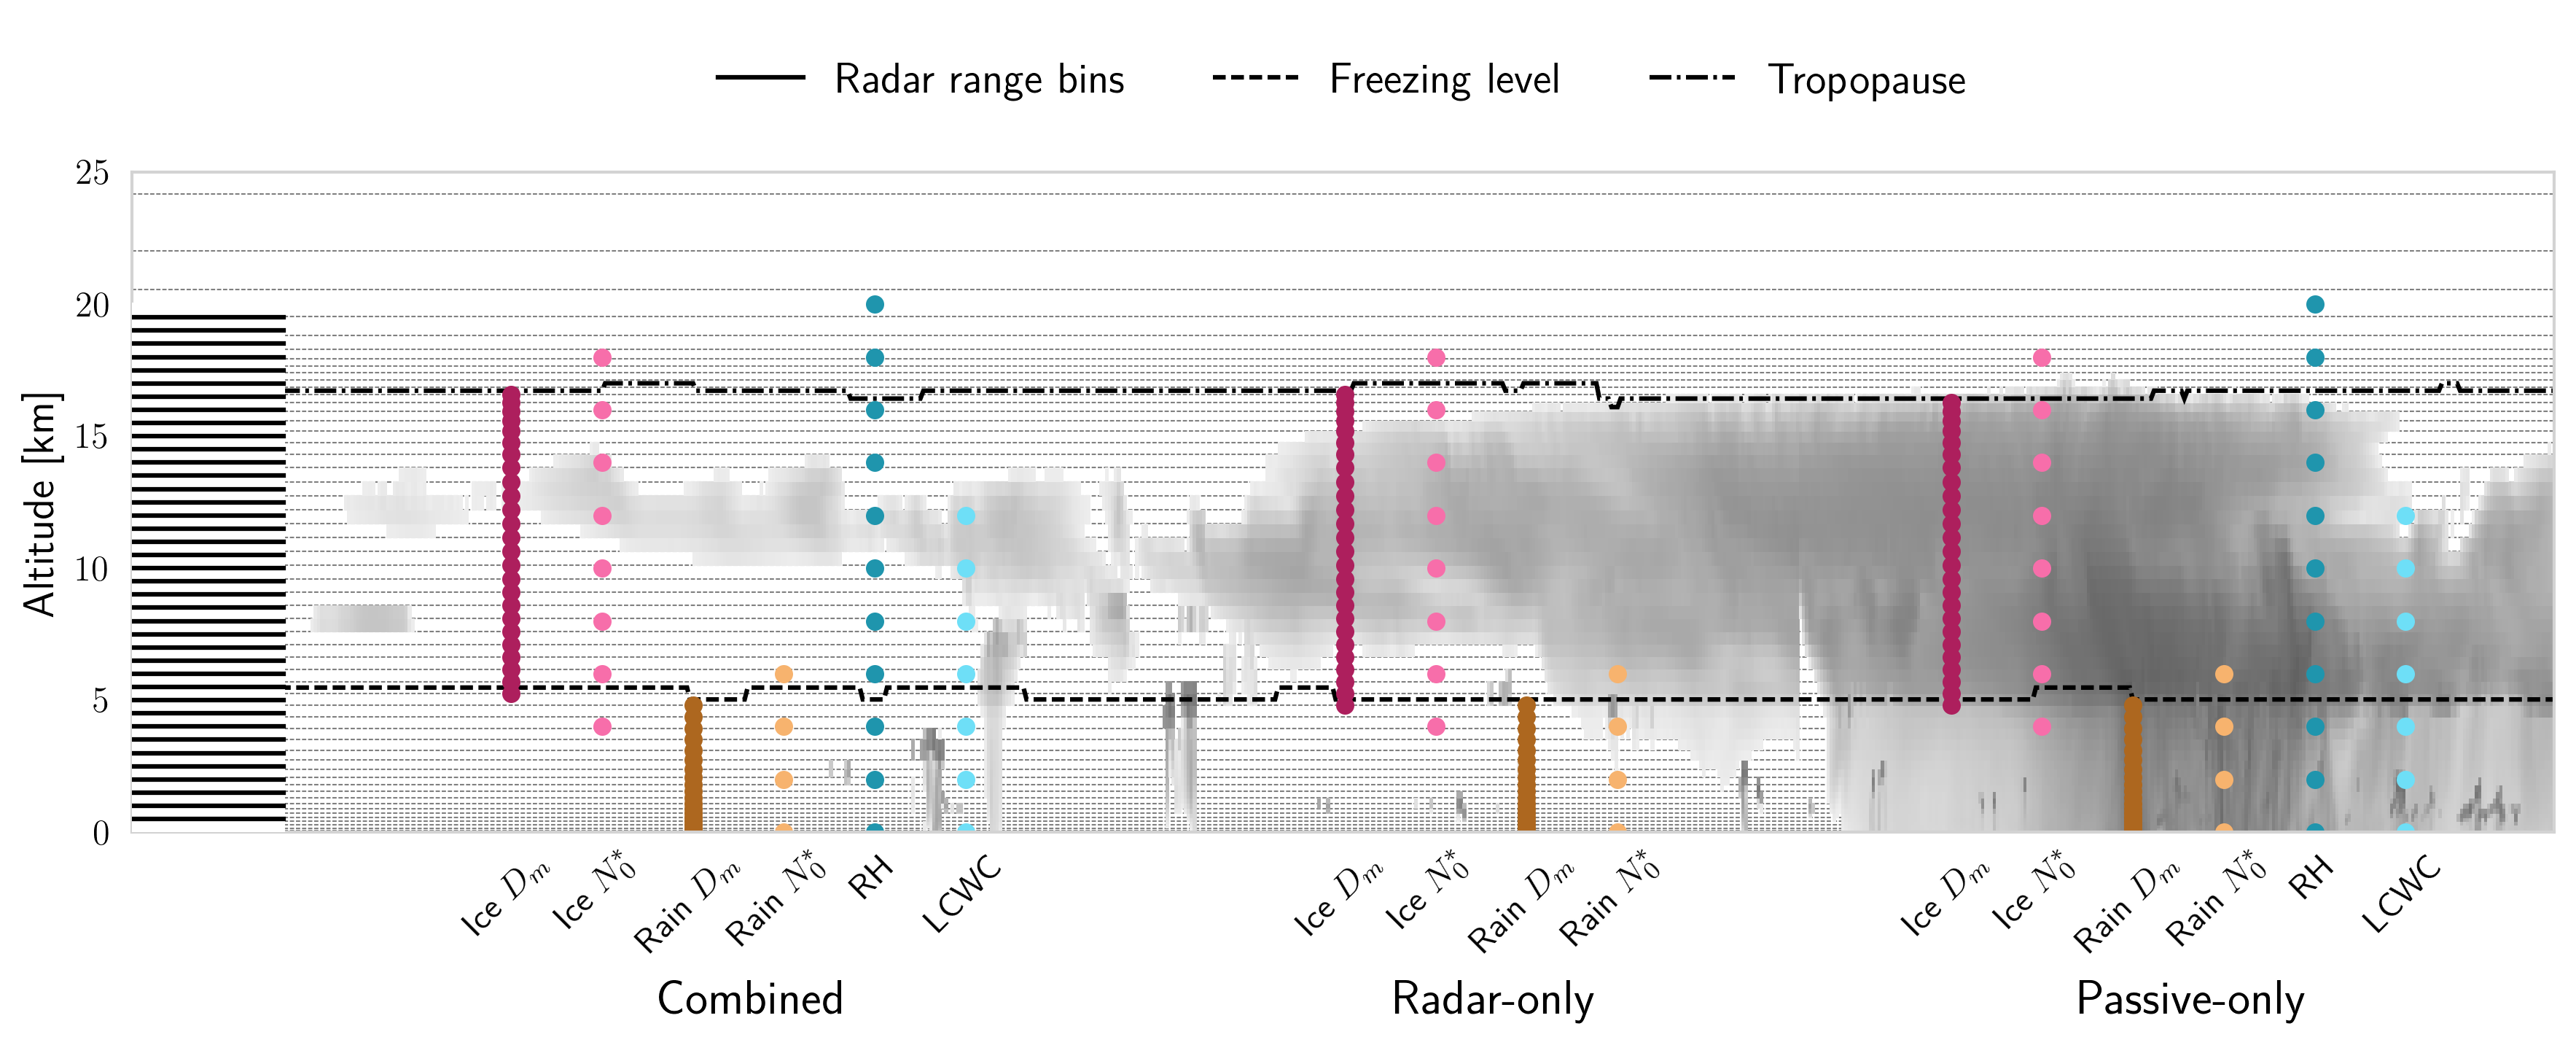
\includegraphics[width = 1.0\linewidth]{../plots/retrieval_sketch}
%\caption{\DIFaddFL{Illustration of the retrieval quantities and their respective retrieval
%  grids. Grey, dashed lines in the background display the vertical grid of the GEM
%  model.  Filled markers represent the retrieval grids of each retrieval quantity
%  for the combined, radar-only and passive-only retrieval.}}
%\label{fig:retrieval_sketch}
%\end{center}
%\end{figure}

\subsection{Reviewer comment}

7. Line 256: Actually, this is only one example of how the radar and radiometer
measurements can be complementary. Even if the lines were parallel (and thus no
information distinguishing size from concentration could be obtained), the radar
still locates the cloud and describes its vertical structure. One can imagine a
cloud of the same ice water path and particle size at two different heights
having different brightness temperatures due to changes in the water vapor
absorption above the cloud – having the radar information would provide increased
information content about the ice water pathin this case than the radiometer
measurement alone.

\subsubsection*{Author response}

It is certainly correct that when a radar sensor is added to a passive
observation system one of the advantages will be the increased resolution.
However, the question that we are interested in are the advantages that neither
of the two instruments can provide on its own. If it was only about vertical
resolution, then the radar alone would be the ideal observation system. In this
case there would be no point in having a satellite that actually flies in
constellation with MetopSG to provide co-located observations. In this sense, we
do not consider the vertical resolution a synergy of the two sensors.

To make this clear, we will add an explanation of our definition of synergies
between the active and passive observations to the section which discusses the
complementary information content.


%Although this is certainly one advantage of combining radar and radiometer
%observations, we do not consider this a true synergy of the active and passive
%observations since correctly locating the cloud in the atmosphere is something
%that the radar can do alone. For the passive to add benefit to the radar, the
%combined observations must provide additional information on the microphysics
%that the radar alone does not provide.


\subsection*{Reviewer comment 8}

Table 4: Why are the values for GemSnow and GemGraupel different than in Table1?

\subsubsection*{Author response}

This was by mistake and will be corrected in the revised version of the
manuscript.

%The differences in the reported values for GemSnow and GemGraupel were due to a
%mistake made by the authors. In the revised version of the manuscript this will
%be corrected and, upon recommendation by reviewer 2, merged into a single table.
%The table now looks as follows:
%
%\begin{table}
%  \begin{center}
%  \caption{\DIFaddFL{Particle model name, ARTS scattering database ID and parameters
%    $\alpha, \beta$ of the mass-size relationships of the particle habits used
%    in the retrieval.}}
%  \begin{tabular}{l|c|c|c}
%    \DIFaddFL{Name }& \DIFaddFL{ID }& \DIFaddFL{$\alpha$ }& \DIFaddFL{$\beta$ }\\
%    \hline
%    \DIFaddFL{LiquidSphere }& \DIFaddFL{25 }& \DIFaddFL{523.6 }& \DIFaddFL{3 }\\
%    \DIFaddFL{GemCloudIce          }& \DIFaddFL{11  }& \DIFaddFL{440      }& \DIFaddFL{3 }\\
%    \DIFaddFL{GemSnow              }& \DIFaddFL{32  }& \DIFaddFL{24  }& \DIFaddFL{2.86 }\\
%    \DIFaddFL{GemGraupel           }& \DIFaddFL{33  }& \DIFaddFL{172.7527 }& \DIFaddFL{2.9646 }\\
%    \DIFaddFL{GemHail              }& \DIFaddFL{34  }& \DIFaddFL{3.02 }& \DIFaddFL{2.9646 }\\
%    \hline
%    \DIFaddFL{SectorSnowflake      }&  \DIFaddFL{3 }& \DIFaddFL{0.0008   }& \DIFaddFL{1.44 }\\
%    \DIFaddFL{8-ColumnAggregate    }&  \DIFaddFL{8   }& \DIFaddFL{65       }& \DIFaddFL{3 }\\
%    \DIFaddFL{LargeColumnAggregate }&  \DIFaddFL{18 }& \DIFaddFL{0.25     }& \DIFaddFL{2.43 }\\
%    \DIFaddFL{LargePlateAggregate  }&  \DIFaddFL{20 }& \DIFaddFL{0.21     }& \DIFaddFL{2.26 }\\
%    \DIFaddFL{IceSphere            }&  \DIFaddFL{24 }& \DIFaddFL{2.2571   }& \DIFaddFL{0.2085 }\\
%  \end{tabular}
%  \label{tab:particle_properties}
%\end{center}
%\end{table}

\subsection*{Reviewer comment 9}

Figures 7 and 8:  I’m not sure why these are separate figures – it seems like all panels could fit on one page.

\subsubsection*{Author response}

Figures 7 and 8 will be combined into a single figure in the revised
manuscript.

%The figure 7 and 8 will be combined into a single figure in the revised version
%of the manuscript:
%
%\begin{figure}
%\begin{center} \DIFdelbeginFL %DIFDELCMD < \includegraphics[width = 0.8\textwidth]{figures/fig07}
%%DIFDELCMD < %%%
%\DIFdelendFL \DIFaddbeginFL 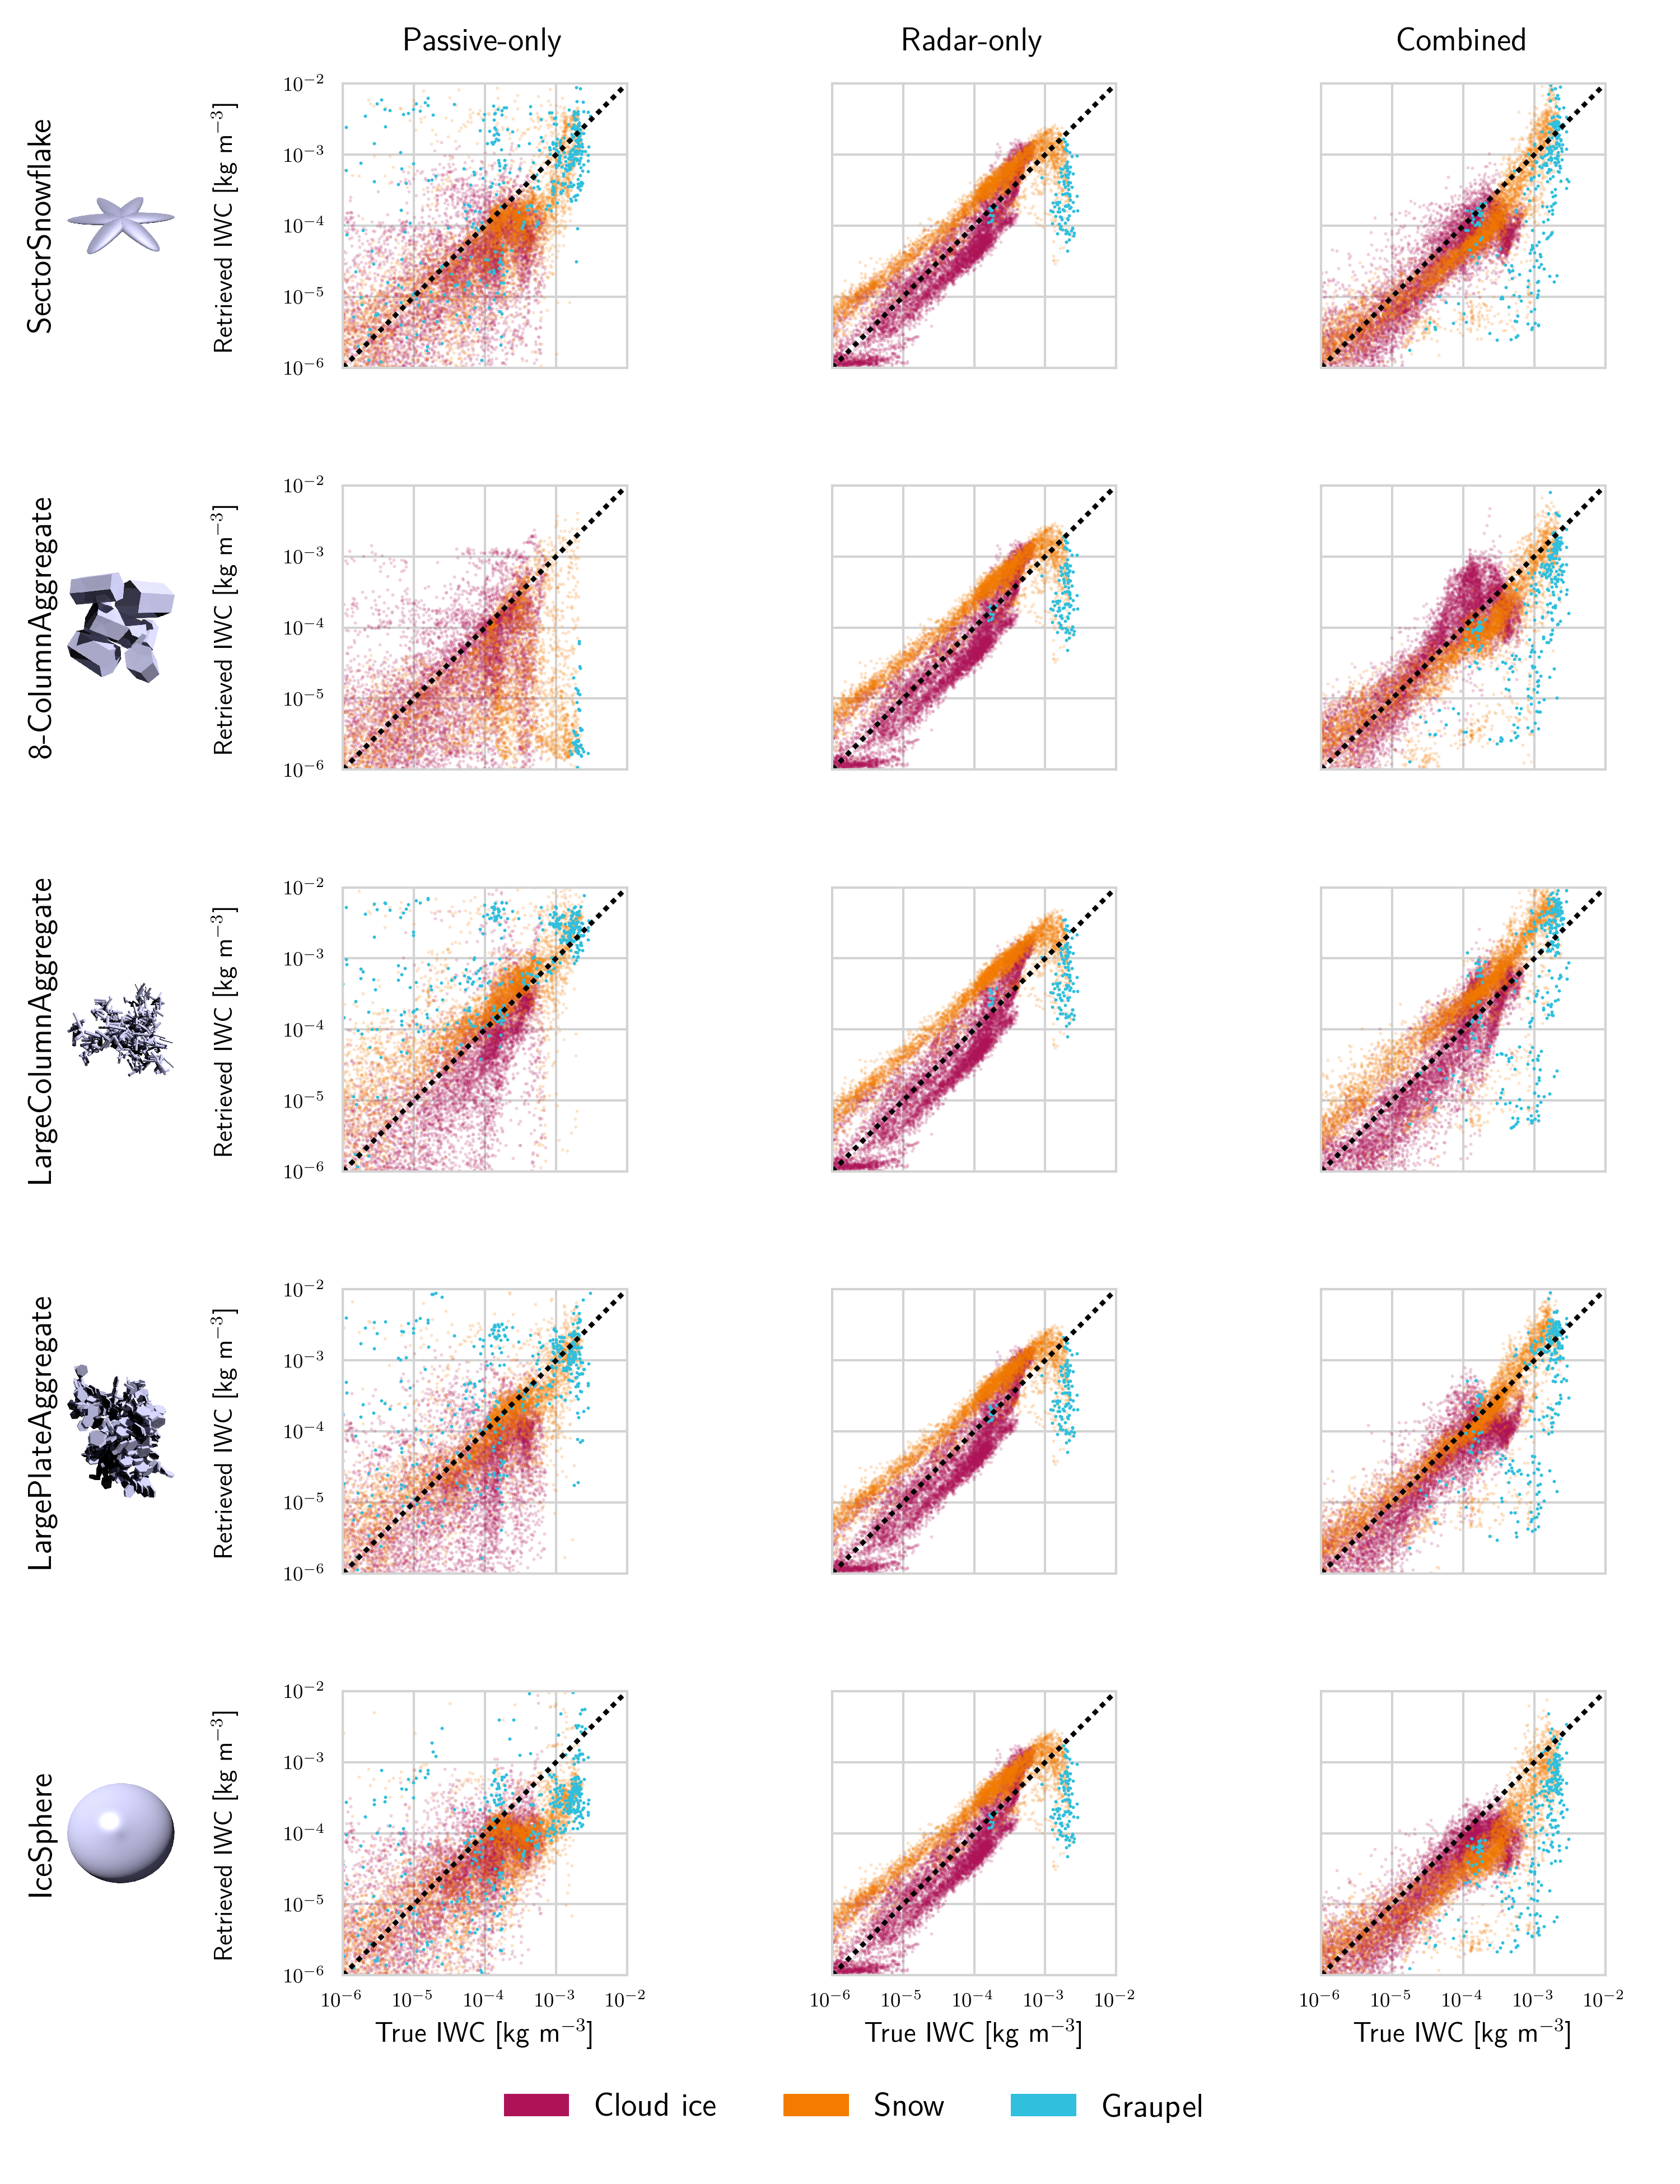
\includegraphics[width = 0.75\textwidth]{../plots/results_scatter_a}
%\DIFaddendFL \caption{\DIFdelbeginFL \DIFdelFL{Reference }\DIFdelendFL \DIFaddbeginFL \DIFaddFL{Retrieved }\DIFaddendFL IWC plotted against \DIFdelbeginFL \DIFdelFL{retrieved }\DIFdelendFL \DIFaddbeginFL \DIFaddFL{reference }\DIFaddendFL IWC for the tested retrieval
%  configurations. Each row shows the retrieval results for the particle shape
%  shown in the first panel. The following panels show the retrieval results for
%  the passive only (first column), the radar only (second column) and the
%  combined retrieval (third column). Markers are colored according to the
%  prevailing hydrometeor type at the corresponding grid point in the test
%  scene. Due to their sparsity, markers corresponding to graupel are drawn at
%  twice the size of the other markers.}
%\DIFdelbeginFL %DIFDELCMD < \label{fig:results_scatter_a_1}
%%DIFDELCMD < %%%
%\DIFdelendFL \DIFaddbeginFL \label{fig:results_scatter_a}
%\DIFaddendFL \end{figure}
%\end{center}

\subsection*{Reviewer comment 11.}
 Line 374: recommend using “represent” instead of “predict”

\subsubsection*{Author response}

The proposed change will be adopted in the updated version of the manuscript.

%\begin{change}[374]
%Since snow will have the
%stronger impact on the observations, the retrieval in these regions tends to
%\DIFdelbegin \DIFdel{predict }\DIFdelend \DIFaddbegin 
%\end{change}

\subsection*{Reviewer commene 12}

 Line 382: should be “reference” instead of “references”

\subsubsection*{Author response}
This will be corrected in the updated version of the manuscript.

% \begin{change}[382]
% The radar-only retrieval does not exhibit any retrieval skill, hardly
% reproducing any of the variation of the \DIFdelbegin \DIFdel{references
% }\DIFdelend \DIFaddbegin \DIFadd{reference }\DIFaddend values. Contrary to
% this, the combined retrieval moves both clusters towards the diagonal,
% indicating that it is capable of distinguishing the microphysical properties of
% cloud ice and snow.
% \end{change}

\subsection*{Reviewer comment 13}

Line  414:  How  are  the  truncated  PSDs  (using  GemSnow)  represented  in  theforward simulations? Is total ice water content conserved? If so, how is it spread amongthe valid particle sizes – equally, or is the truncated mass allocated to the smallest size bin?

\subsubsection*{Author response}

Total IWC is not conserved in the handling of PSDs. The point raised by the reviewer has been
investigated by assessing the effect of the truncation on the water content of snow in the
forward simulations. The results of the analysis are given in the figure below. As these results
show, the effects of the truncation in the forward simulations are negligible.

However, when the GemSnow particle model is used in the retrieval it can
introduce significant errors. For this reason as well as another reviewers'
comment regarding the choice of tested particles, the selection of particles to
be used in the retrieval will be changed for the revised manuscript and the
GemSnow particle will not be included. Instead, only particle models will be used
that cover all relevant particles sizes.

\begin{figure}[!hbpt]
  \begin{center}
  \includegraphics[width = 1.0\textwidth]{../plots/truncated_iwc}
  \caption{Joint distribution of truncated and full snow water content (SWC) for the
    two test scenes.}
  \end{center}
\end{figure}

\subsection*{Reviewer comment 14}

Figure 16: The figure labels/captions aren't clear if they refer to total liquid water
content/path or just the cloud liquid water/path.

\subsubsection{Author response}

We will clarify that the contours refer to liquid cloud water content in the revised
version of the manuscript.

\subsection*{Reviewer comment 15}

 Line 518: It’s interesting that the Plate Aggregate provides the most accurate
 re-trieval results, even though it isn’t similar to the models used in the
 synthetic measure-ment simulations. Does the decreasing density with size
 better replicate the combina-tion of high-density GemCloudIce (which tends to
 be present in high concentrations atsmall sizes) and lower-density GemSnow
 (which tends to be dominant at larger sizes)?

\subsubsection{Author response}
Unfortunately, we cannot give a definitive answer to this question. As panel (a) in Fig. 15
shows, the density of the LargePlateAggregate habit is actually lower than that of snow for
large particle sizes. Moreover, the scattering properties certainly also play a role here.
It is therefore difficult to postulate any direct causality between the particle density and
the performance in the retrieval.

\bibliographystyle{copernicus}
\bibliography{references}



\end{document}
